\chapter{Introduction}\label{chapter:intro}
\section{Problem}
Nowadays, data in the internet has gone from scarce to superabundant. This brings us huge new advantages, but also challenges\cite{1_the_economist_2010}. The cyber world contains a large amount of digital data which is constantly changing and getting ever vaster. This makes the raw data widely available everywhere. Meanwhile, the ability of extracting knowledge from the multifarious data becomes desperately needed. ``Researchers need to adapt their institutions and practices in response to torrents of new data — and need to complement smart science with smart searching'', says Nature\cite{Nature:2008jh}.

However, most data on the internet is unstructured, littery and dynamic. Furthermore, they are often wrapped into very different and complicated modes of presentation. When trying to do some automatic search on a specific topic, artificial intelligence will face huge challenges.\\

\noindent There are three scenarios in the real world:
\begin{enumerate}
  \item When a high school student applying for an undergraduate programme, he may need to collect and compare the information of different programmes in different departments and different universities. It includes but not limited to selection criteria, funding, tuition fee and how to apply. However, the introductions to these programmes are on different webpages and share disparate layouts. Thus, the student needs to spend a large amount of time to integrate information about the programmes such as course structure and entry requirement. Furthermore, some information such as course introduction may only exists in PDF files, which makes automatic information extraction even harder.
  \item Another example is looking for the information of current and up-coming art	exhibitions around the country. The exhibitions' open hours and dates could be shown anywhere in diverse forms. For example, on the an exhibition's own website and the various city council's website. It might also have different prices for the tickets, for instance, a person who has a membership may be eligible to enjoy a discount on price. Moreover, the information found might be duplicate, which makes the arrangements of visiting art exhibitions even harder.
  \item Looking up research papers is also an example. When doing literature review, a researcher is usually required to loop up to a large amount of research papers. Nowadays, most of the recent papers could be found online. However, the research papers appear on various websites and are often in PDF format. And one research paper may exists on many different websites. Though based information of these paper are structured, they may have very different webpage layouts. Thus, it is difficult that we build a large database to manage the information and make it convenient for researchers to use.
\end{enumerate}

Hence, this kind of problems have been hard to solve so far. It is mainly because that the semantic web is still not mature and web is based on normal html content. However, these massive layouts make it difficult to integrate structured and logical data. Meanwhile, in order to achieve semi-automation, it is required to pick out the webpage with target information among the large amount of chaotic webpages. Thus, implementing a web page filter is also a big challenge that cannot be ignored.

\section{Case Study: Oxford Seminar Announcements}

The scenarios we stated above might be too large, and the correctness of the result is hard to test. Thus, we decide to choose a relatively small but representative problem in a specific domain for this project. As seminar announcements in the University of Oxford is very typical, we will use it as our case study. Additionally, it is very practical and useful to develop such a system for fellows and students in the University of Oxford.

\begin{figure}[htb!]
	\centering
	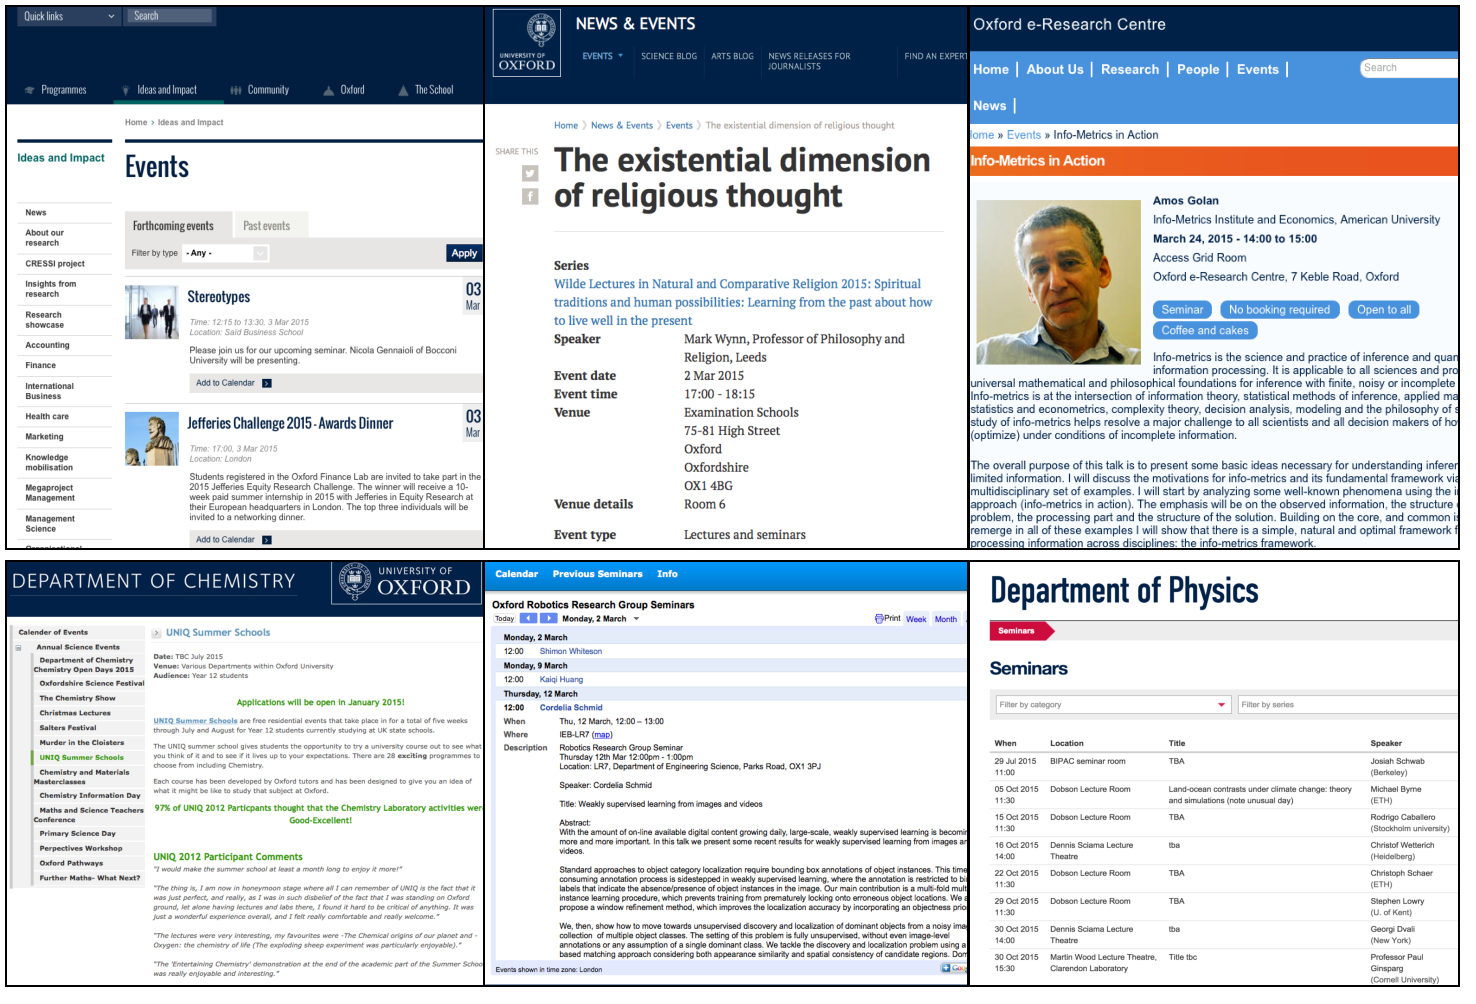
\includegraphics[page=1,width=\textwidth]{images/picture.pdf}
	\caption{Sample Seminar Announcement Pages in University of Oxford Websites}\label{fig:emp:various_layout}
\end{figure}

There are numerous seminar announcements in University of Oxford each week, and they are structured very differently and exhibits in various forms(as shown in Figure \ref{fig:emp:various_layout}). The majority of 395 departments and 38 colleges have their own website\footnote{data is obtained from University of Oxford official website}, and most of them has its own way to display seminar information. A rough statistics shows that currently there are approximately 2000 seminars taking place in Oxford every month\footnote{data is estimated by the google search result}. Filtering out the related web pages, extracting required data and visualising seminar information from such a huge amount of web pages is a very difficult and complicated process. And seminar information updates frequently, which makes demands on high efficiency. It can hardly be done by human beings manually. 

Therefore, the system we developed here should be capable of filtering seminar announcement pages from the given domain, dynamically collecting seminar information each week throughout the billions of Oxford web pages and present them in numerous visualisation forms.

\section{Aims and Objectives}
The purpose of this project is to design and develop an semi-automatic system to solve such complex problem. The system covers the entire process from data collecting at the beginning and data presentation at last. It needs to do web page classification based on machine learning and human interaction. Meanwhile, it is able to capture information and generate corresponding tabular data from the given domains, and provide a visualisation to show the result knowledge for the end users by using state of art technologies. Both web page classification and information extraction are completed with the help of visual analytics. In general, it is the process of ontology-based visual analytics for text analysis.

In particular, considering our study case, the entire project is required to achieve the following objectives:
\begin{itemize}
	\item Implement an intelligent crawler to conduct web crawling in the University of Oxford's website;
	\item Design and implement an ontology-based automatic web page filter to pick out all the target webpages that contain seminar announcement;
	\item Create data sets for seminar announcement pages;\footnote{There is no existing data set for seminar announcement pages, we should create it by ourself manually.}
	\item Design and conduct experiments to test the web page classification above by using the data sets;
	\item Design and implement a semi-automatic solution to extract the seminar announcement information from the target webpages under the assistance which combining ontology and visual analytics.
	\item Design and implement a visualisation to present a large number of seminar announcements;
	\item Create a pipeline and implement a complete and feasible system to combine all the function above together to form a systematic solution.
\end{itemize}

\section{Setting and Assumption}
\begin{enumerate}
	\item Domain\\
	This project will constraint the targets within the domain of \code{ox.ac.uk}, i.e. all webpages in this domain will be covered in this project.
	\item Target Entity\\
	Seminar announcement information is regarded as the target entity.
	A seminar announcement page is a web page that contains at least one announcement for a seminar.
	According to the Merriam-Webster Dictionary, a `seminar' is `
	\begin{enumerate*}[label=\textit{(\arabic*)}]
		\item \textit{a meeting in which you receive information on and training in a particular subject;}
		\item \textit{a class offered to a small group of students at a college or university}
	\end{enumerate*}'.
	An `announcement' is `\textit{a written or spoken statement that tells people about something: public or formal words that announce something}'\cite{merriam2004merriam}.
	
	Therefore, a seminar announcement in Oxford is a statement which tells people about information related to a short training or meeting in the University of Oxford. It must contain at least the following facts related to a seminar: 
	\begin{center}
		date, time, location, subject, speaker
	\end{center}
	It may also contain information about:
	\begin{center}
		target audience, abstract of seminar, short introduction of speaker, \\
		how to book, organiser, seminar frequency
	\end{center}	
	
	\item Attribute\\
	Based on the study on a large number of seminar announcement pages on the Oxford websites, we decided to select the following attributes of seminar announcement in research:
	\begin{center}
		date, time, title, location, speaker, abstract		
	\end{center}
	It contains format information including string, time and date.
	\item Dynamic Page Techniques\\
	Here, we do not consider the various webpage structures generated by the front-end dynamic page technologies such as Ajax, AngularJS\cite{mesbah2012crawling, grant2014basics}. Because in order to construct these webpages, we need to implement a browser kernel to parse and execute javascript. However, this project focuses on using ontologies and visual analytics to do semi-automatic webpage classification and information extraction. As time is limited, we decide to ignore these kinds of dynamic pages.
\end{enumerate}


\section{Dissertation Structure}
In this dissertation, we will first give a brief introduction to the problem we are going to solve, especially why we have this problem and what is our study case.

Next, we will give the background study and literature review for the project in chapter \ref{chapter:bg}. First of all, we will briefly introduce the wide background knowledge related to our solution. Secondly, there will be a short discussion about the related research and solutions so far.

In chapter \ref{chapter:solution}, we will state a formal setting of the problem we are facing and give an overview of the solution. The key issues and main challenges will be described here. There will also be an explanation to the whole solution pipeline of this ontology-based visual analytics for text analysis.

In the following chapter \ref{chapter:clf} and chapter \ref{chapter:ie}, an explanation of the core parts in our solution, webpage classification and information extraction, will be delivered in details. It helps with showing the readers what are the advantages of this solution.

Last but not least, there will be a critical thinking part about further study and conclusion. We will give the adaptability of the solution and some possible applications in other areas.
